% Fig. 1 — NPU-hardened LiSenNet architecture (standalone TikZ -> architecture.pdf).
% Build: pdflatex architecture.tex   (run from paper/figures/)
% Design: two-row U-Net snake (encoder top, decoder bottom, vertically aligned
% skips), dual-path conv bottleneck expanded in a detail panel below.
% Colors validated CVD-safe (dataviz skill): blue = the conv redesign,
% orange = hardening swaps, violet = FIFO streaming state.
\documentclass[tikz,border=2pt]{standalone}
\usepackage{times}
\usepackage{amsmath}
\usetikzlibrary{positioning,calc,arrows.meta,fit}

% palette (validated)
\definecolor{convblue}{HTML}{2A78D6}
\definecolor{hardorange}{HTML}{EB6834}
\definecolor{stviolet}{HTML}{4A3AA7}

\begin{document}
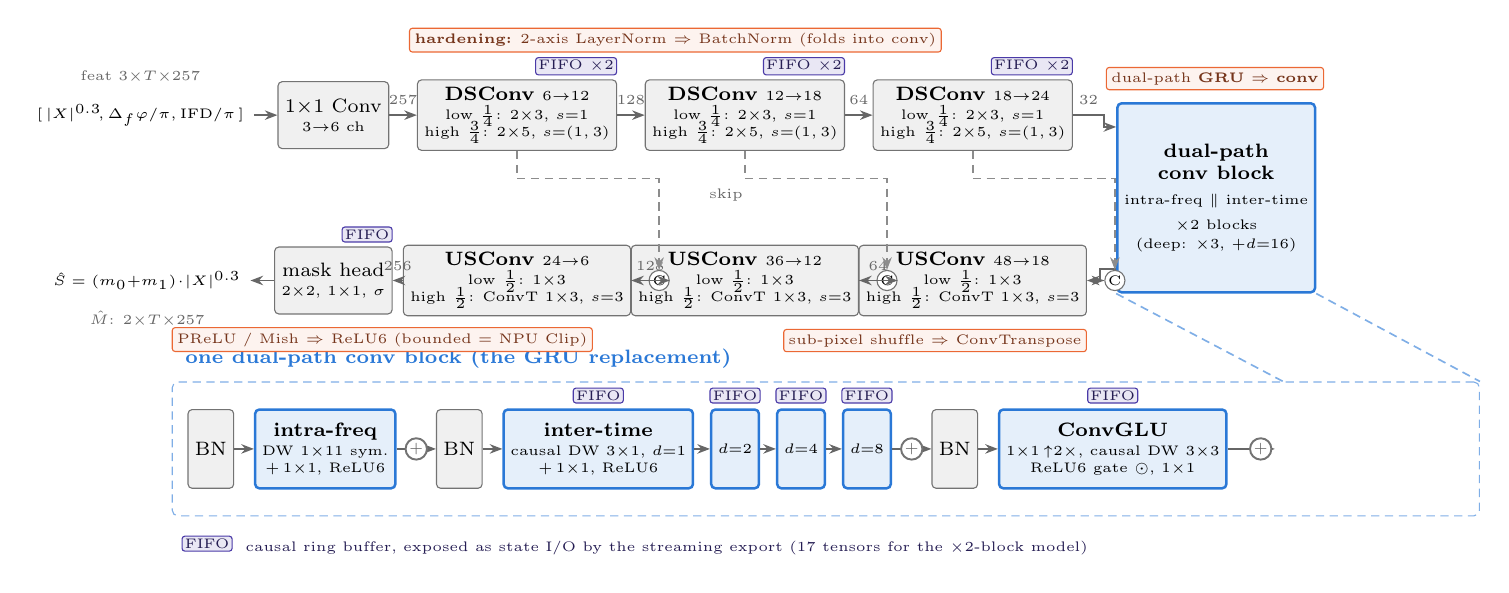
\begin{tikzpicture}[
  font=\scriptsize,
  >={Stealth[length=1.6mm]},
  flow/.style={->, black!60, line width=0.7pt},
  skip/.style={->, black!45, densely dashed, line width=0.6pt},
  blk/.style={draw=black!55, fill=black!6, rounded corners=1.5pt,
              align=center, inner sep=2.5pt, minimum height=8.5mm},
  ds/.style={blk, minimum width=20mm},
  bneck/.style={draw=convblue, fill=convblue!12, rounded corners=1.5pt,
                align=center, inner sep=2.5pt, line width=0.9pt},
  swap/.style={draw=hardorange, fill=hardorange!8, rounded corners=1pt,
               align=left, inner sep=1.8pt, font=\tiny, text=hardorange!50!black},
  fifo/.style={draw=stviolet, fill=stviolet!12, rounded corners=1pt,
               inner sep=1pt, font=\tiny, text=stviolet!50!black},
  cc/.style={draw=black!55, fill=white, circle, inner sep=0.5pt, font=\tiny},
  lbl/.style={font=\tiny, text=black!60},
]

% =========================== encoder row (top) ==============================
\node[blk, minimum width=12mm] (c1) at (0,0) {$1{\times}1$ Conv\\[-1pt]{\tiny $3{\to}6$ ch}};
\node[ds, right=3.5mm of c1] (d1) {\textbf{DSConv} {\tiny $6{\to}12$}\\[-1pt]
  {\tiny low $\tfrac14$: $2{\times}3$, $s{=}1$}\\[-2pt]
  {\tiny high $\tfrac34$: $2{\times}5$, $s{=}(1,3)$}};
\node[ds, right=3.5mm of d1] (d2) {\textbf{DSConv} {\tiny $12{\to}18$}\\[-1pt]
  {\tiny low $\tfrac14$: $2{\times}3$, $s{=}1$}\\[-2pt]
  {\tiny high $\tfrac34$: $2{\times}5$, $s{=}(1,3)$}};
\node[ds, right=3.5mm of d2] (d3) {\textbf{DSConv} {\tiny $18{\to}24$}\\[-1pt]
  {\tiny low $\tfrac14$: $2{\times}3$, $s{=}1$}\\[-2pt]
  {\tiny high $\tfrac34$: $2{\times}5$, $s{=}(1,3)$}};

% =========================== bottleneck (right, spans rows) =================
\node[bneck, minimum width=21mm, minimum height=24mm, anchor=west]
      (bn) at ($(d3.east)+(5.5mm,-1.05)$)
      {\textbf{dual-path}\\\textbf{conv block}\\[1pt]
            {\tiny intra-freq $\parallel$ inter-time}\\[1pt]
            {\tiny $\times2$ blocks}\\[-1pt]{\tiny (deep: $\times3$, $+d{=}16$)}};

% =========================== decoder row (bottom) ===========================
\node[ds] (u1) at (d3 |- 0,-2.1) {\textbf{USConv} {\tiny $48{\to}18$}\\[-1pt]
  {\tiny low $\tfrac12$: $1{\times}3$}\\[-2pt]
  {\tiny high $\tfrac12$: ConvT $1{\times}3$, $s{=}3$}};
\node[ds] (u2) at (d2 |- u1) {\textbf{USConv} {\tiny $36{\to}12$}\\[-1pt]
  {\tiny low $\tfrac12$: $1{\times}3$}\\[-2pt]
  {\tiny high $\tfrac12$: ConvT $1{\times}3$, $s{=}3$}};
\node[ds] (u3) at (d1 |- u1) {\textbf{USConv} {\tiny $24{\to}6$}\\[-1pt]
  {\tiny low $\tfrac12$: $1{\times}3$}\\[-2pt]
  {\tiny high $\tfrac12$: ConvT $1{\times}3$, $s{=}3$}};
\node[blk, minimum width=12mm] (mh) at (c1 |- u1)
  {mask head\\[-1pt]{\tiny $2{\times}2$, $1{\times}1$, $\sigma$}};

% concat circles at decoder inputs
\node[cc, right=2.2mm of u1.east] (cat1) {C};
\node[cc, right=2.2mm of u2.east] (cat2) {C};
\node[cc, right=2.2mm of u3.east] (cat3) {C};

% =========================== main flow =======================================
\node[font=\tiny, align=center, left=3mm of c1] (in)
  {$[\,|X|^{0.3}\!,\Delta_f\varphi/\pi,\mathrm{IFD}/\pi\,]$};
\node[lbl, anchor=south] at ($(in.north)+(0,0.2mm)$) {feat $3{\times}T{\times}257$};
\draw[flow] (in) -- (c1);
\draw[flow] (c1) -- node[lbl,above]{257} (d1);
\draw[flow] (d1) -- node[lbl,above]{128} (d2);
\draw[flow] (d2) -- node[lbl,above]{64} (d3);
\draw[flow] (d3.east) -- node[lbl,above]{32} ++(4mm,0) |- ($(bn.west)+(0,9mm)$);
\draw[flow] ($(bn.west)+(0,-9mm)$) -- ++(-2mm,0) |- (cat1);
\draw[flow] (cat1) -- (u1);
\draw[flow] (u1) -- node[lbl,above]{64} (cat2);
\draw[flow] (cat2) -- (u2);
\draw[flow] (u2) -- node[lbl,above]{128} (cat3);
\draw[flow] (cat3) -- (u3);
\draw[flow] (u3) -- node[lbl,above]{256} (mh);
\node[font=\tiny, align=center, left=3mm of mh] (out)
  {$\hat S=(m_0{+}m_1)\!\cdot\!|X|^{0.3}$};
\node[lbl, anchor=north] at ($(out.south)+(0,-0.2mm)$) {$\hat M$: $2{\times}T{\times}257$};
\draw[flow] (mh) -- (out);

% skip connections: drop, then run horizontally mid-gap, then into the concat
\draw[skip] (d3.south) -- ++(0,-3.5mm) -| (cat1);
\draw[skip] (d2.south) -- ++(0,-3.5mm) node[lbl, below left=0mm and -1mm]{skip} -| (cat2);
\draw[skip] (d1.south) -- ++(0,-3.5mm) -| (cat3);

% =========================== detail panel ===================================
\node[draw=convblue!60, densely dashed, rounded corners=2pt, inner sep=3mm,
      minimum width=166mm, minimum height=17mm, anchor=north west]
      (panel) at ($(mh.south west)+(-13mm,-8.5mm)$) {};
\node[font=\scriptsize\bfseries, text=convblue, anchor=south west]
      at ($(panel.north west)+(0.5mm,0.4mm)$) {one dual-path conv block (the GRU replacement)};

% --- intra-frequency group
\node[blk, anchor=west, minimum height=10mm] (bn1) at ($(panel.west)+(2mm,0)$) {BN};
\node[bneck, right=2.5mm of bn1, minimum height=10mm]
  (intra) {\textbf{intra-freq}\\[-1pt]{\tiny DW $1{\times}11$ sym.}\\[-2pt]{\tiny $+\,1{\times}1$, ReLU6}};
% --- inter-time group
\node[blk, right=5mm of intra, minimum height=10mm] (bn2) {BN};
\node[bneck, right=2.5mm of bn2, minimum height=10mm] (it1)
  {\textbf{inter-time}\\[-1pt]{\tiny causal DW $3{\times}1$, $d{=}1$}\\[-2pt]{\tiny $+\,1{\times}1$, ReLU6}};
\node[bneck, right=2mm of it1, minimum height=10mm] (it2) {{\tiny $d{=}2$}};
\node[bneck, right=2mm of it2, minimum height=10mm] (it3) {{\tiny $d{=}4$}};
\node[bneck, right=2mm of it3, minimum height=10mm] (it4) {{\tiny $d{=}8$}};
% --- GLU group
\node[blk, right=5mm of it4, minimum height=10mm] (bn3) {BN};
\node[bneck, right=2.5mm of bn3, minimum height=10mm] (glu)
  {\textbf{ConvGLU}\\[-1pt]{\tiny $1{\times}1\,{\uparrow}2\times$, causal DW $3{\times}3$}\\[-2pt]{\tiny ReLU6 gate $\odot$, $1{\times}1$}};

\draw[flow] (bn1) -- (intra);
\draw[flow] (intra) -- node[cc, pos=0.5, inner sep=0.4pt]{+} (bn2);
\draw[flow] (bn2) -- (it1);
\draw[flow] (it1) -- (it2); \draw[flow] (it2) -- (it3); \draw[flow] (it3) -- (it4);
\draw[flow] (it4) -- node[cc, pos=0.5, inner sep=0.4pt]{+} (bn3);
\draw[flow] (bn3) -- (glu);
\draw[flow] (glu.east) -- node[cc, pos=0.7, inner sep=0.4pt]{+} ++(6mm,0);

% FIFO chips on causal convs (streaming state)
\node[fifo, anchor=south] at ($(it1.north)+(0,0.6mm)$) {FIFO};
\node[fifo, anchor=south] at ($(it2.north)+(0,0.6mm)$) {FIFO};
\node[fifo, anchor=south] at ($(it3.north)+(0,0.6mm)$) {FIFO};
\node[fifo, anchor=south] at ($(it4.north)+(0,0.6mm)$) {FIFO};
\node[fifo, anchor=south] at ($(glu.north)+(0,0.6mm)$) {FIFO};
% and on the encoder/decoder causal convs
\node[fifo, anchor=south east] at ($(d1.north east)+(0,0.5mm)$) {FIFO $\times2$};
\node[fifo, anchor=south east] at ($(d2.north east)+(0,0.5mm)$) {FIFO $\times2$};
\node[fifo, anchor=south east] at ($(d3.north east)+(0,0.5mm)$) {FIFO $\times2$};
\node[fifo, anchor=south east] at ($(mh.north east)+(0,0.5mm)$) {FIFO};

% zoom bracket: bottleneck -> panel
\draw[convblue!60, densely dashed, line width=0.6pt]
  (bn.south west) -- ($(panel.north east)+(-25mm,0)$);
\draw[convblue!60, densely dashed, line width=0.6pt]
  (bn.south east) -- (panel.north east);

% =========================== hardening callouts ==============================
\node[swap, anchor=south west] at ($(d1.north west)+(-1mm,3.4mm)$) (sw1)
  {\textbf{hardening:} 2-axis LayerNorm $\Rightarrow$ BatchNorm (folds into conv)};
\node[swap, anchor=south east] at ($(bn.north east)+(1mm,1.5mm)$) (sw2)
  {dual-path \textbf{GRU} $\Rightarrow$ \textbf{conv}};
\node[swap, anchor=north east] at ($(u1.south east)+(0,-1.6mm)$) (sw3)
  {sub-pixel shuffle $\Rightarrow$ ConvTranspose};
\node[swap, anchor=north west] at ($(mh.south west)+(-13mm,-1.6mm)$) (sw4)
  {PReLU / Mish $\Rightarrow$ ReLU6 (bounded $=$ NPU Clip)};

% legend (violet)
\node[font=\tiny, text=stviolet!50!black, anchor=north west]
  at ($(panel.south west)+(0,-1.2mm)$)
  {\tikz\node[fifo]{FIFO};\ \ causal ring buffer, exposed as state I/O by the
   streaming export (17 tensors for the $\times2$-block model)};

\end{tikzpicture}
\end{document}
